\section{Desarrollo de la propuesta}

\subsection{Estrategia experimental}

La etapa experimental se estructuro en cinco experimentos secuenciales: \textit{baseline}, \textit{agregaciones}, \textit{categorizaciones}, \textit{pruning} e \textit{hiperparametros}. Esta nomenclatura coincide con el flujo de experimentacion definido para la sustentacion.

Todas las metricas reportadas en esta seccion se obtienen directamente de los metadatos generados por el pipeline, usando como fuente primaria:

\begin{itemize}
\item \texttt{doc/experiments/exp\_0X\_*/comparison\_plots/comparison\_metadata.json} para AUC comparativo entre modelos.
\item \texttt{doc/experiments/exp\_05\_hyperparameter\_search/models/<modelo>/plots/plot\_metadata.json} para metricas operativas del duelo final (threshold, recall, specificity, precision, NPV, F1, F2, accuracy, kappa).
\end{itemize}

\subsection{Experimento 1: Baseline}

En el experimento baseline se evaluaron siete algoritmos con configuracion base para establecer la linea de referencia.

\begin{table}[H]
\centering
\caption{Top 3 modelos por AUC-ROC en el Experimento 1}
\label{tab:exp1-top3}
\begin{tabular}{|l|c|}
\hline
\textbf{Modelo} & \textbf{AUC-ROC} \\ \hline
catboost & 0.6153 \\ \hline
logistic\_regression\_lasso & 0.6055 \\ \hline
xgboost & 0.5950 \\ \hline
\end{tabular}
\end{table}

\begin{figure}[H]
\centering
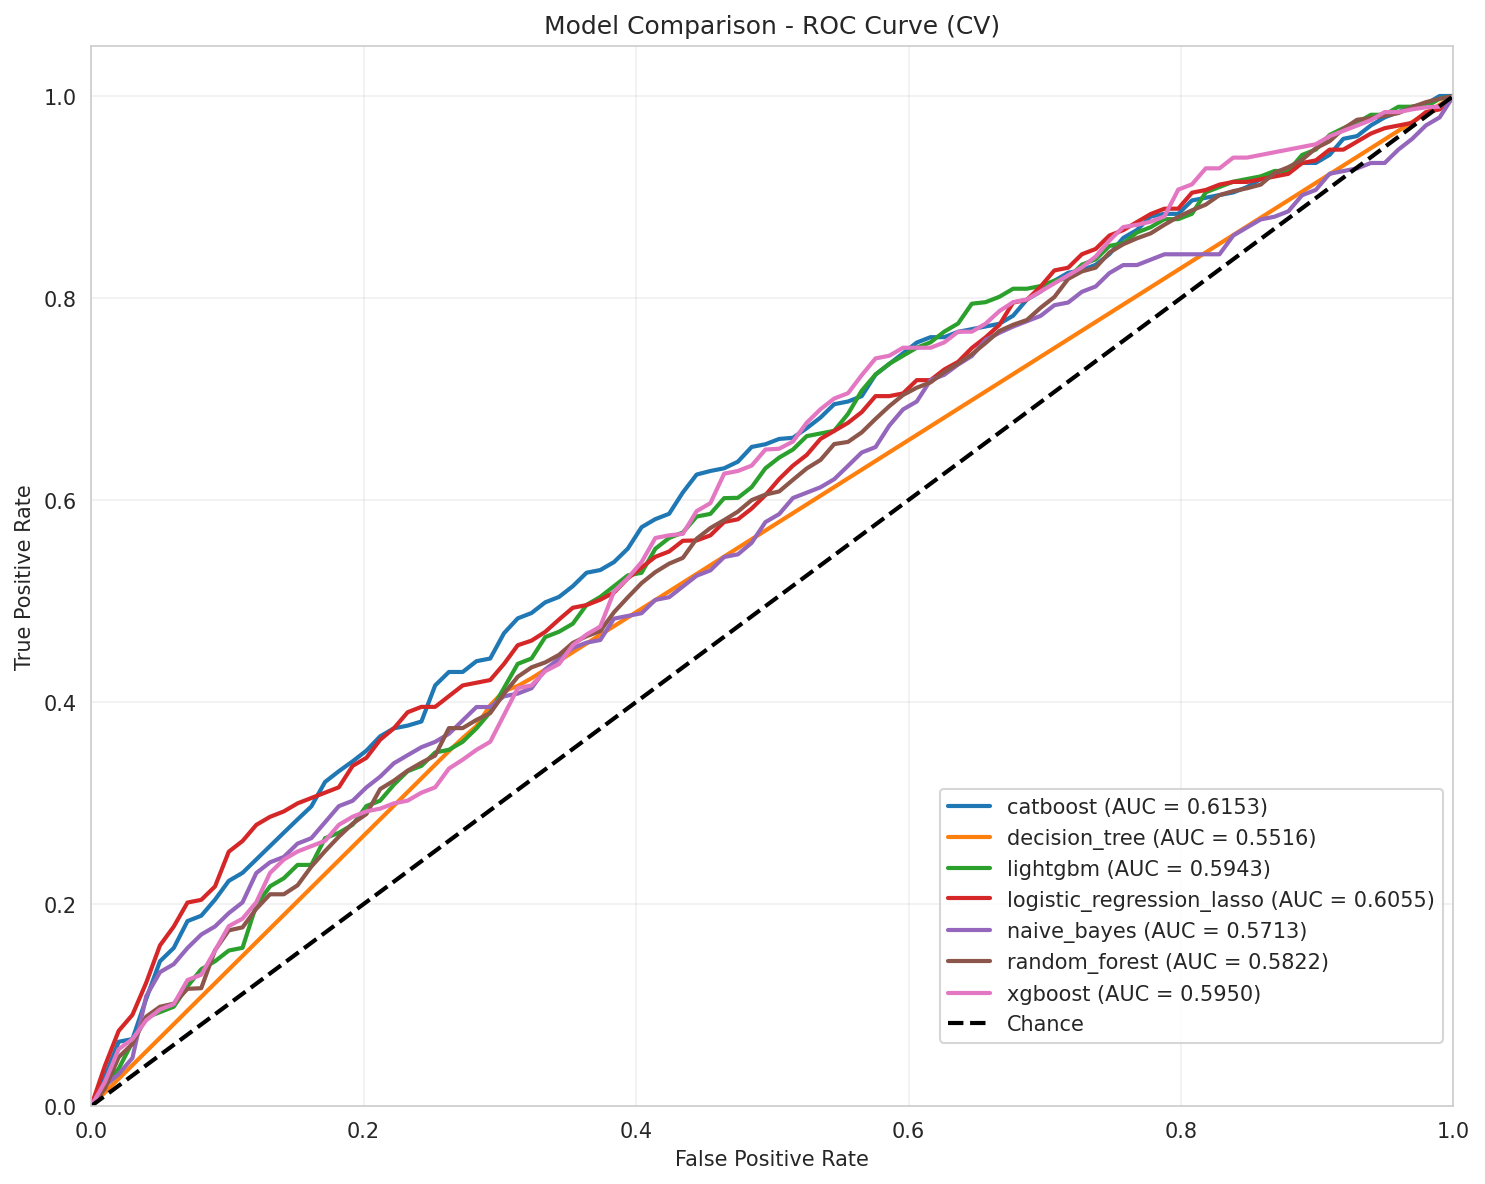
\includegraphics[width=0.85\textwidth]{../experiments/exp_01_base_models/comparison_plots/roc_comparison.png}
\caption{Comparacion ROC global del Experimento 1}
\label{fig:exp1-roc}
\end{figure}

\begin{figure}[H]
\centering
\includegraphics[width=0.78\textwidth]{../experiments/exp_01_base_models/models/catboost/plots/feature_importance.png}
\caption{Importancia de variables del modelo lider (catboost) en el Experimento 1}
\label{fig:exp1-fi-catboost}
\end{figure}

\subsection{Experimento 2: Agregaciones}

Se incorporaron variables derivadas y agregaciones clinicas para aumentar la capacidad discriminativa del modelo. El mejor resultado de esta fase fue catboost con AUC-ROC de 0.6235.

\begin{table}[H]
\centering
\caption{Top 3 modelos por AUC-ROC en el Experimento 2}
\label{tab:exp2-top3}
\begin{tabular}{|l|c|}
\hline
\textbf{Modelo} & \textbf{AUC-ROC} \\ \hline
catboost & 0.6235 \\ \hline
logistic\_regression\_lasso & 0.6044 \\ \hline
lightgbm & 0.5969 \\ \hline
\end{tabular}
\end{table}

\begin{figure}[H]
\centering
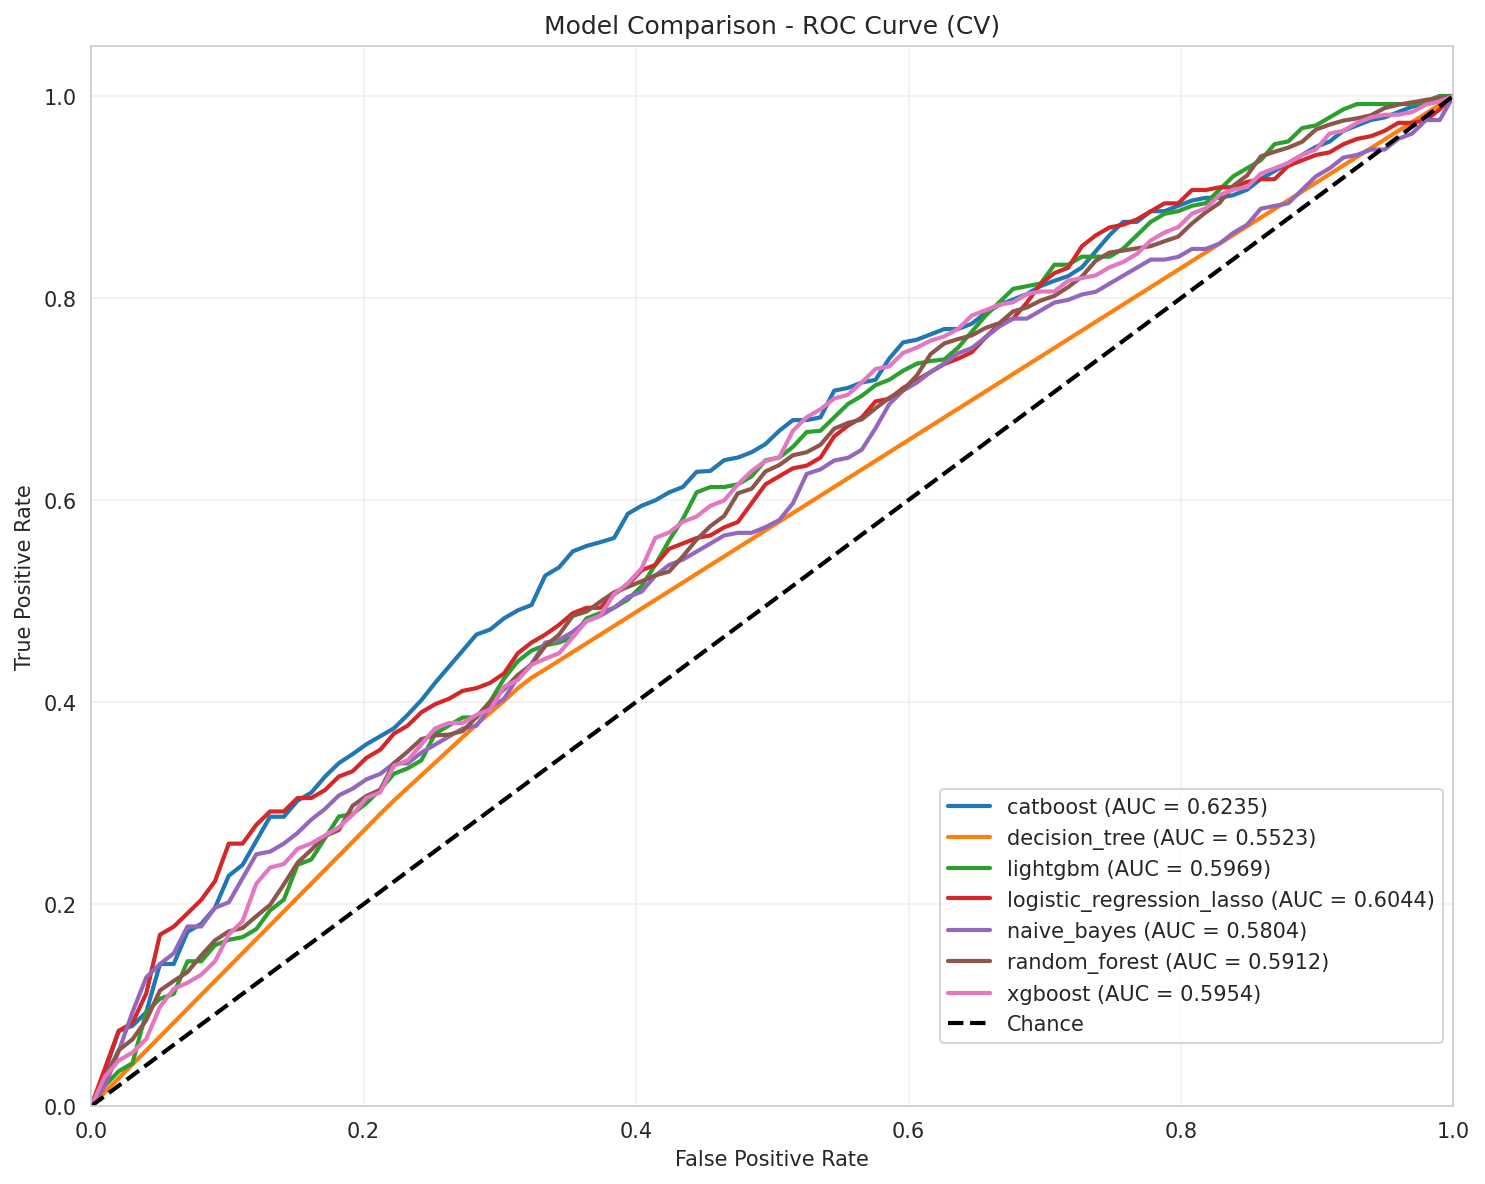
\includegraphics[width=0.85\textwidth]{../experiments/exp_02_aggregated_features/comparison_plots/roc_comparison.png}
\caption{Comparacion ROC global del Experimento 2}
\label{fig:exp2-roc}
\end{figure}

\begin{figure}[H]
\centering
\includegraphics[width=0.78\textwidth]{../experiments/exp_02_aggregated_features/models/catboost/plots/feature_importance.png}
\caption{Importancia de variables del modelo lider (catboost) en el Experimento 2}
\label{fig:exp2-fi-catboost}
\end{figure}

\subsection{Experimento 3: Categorizaciones}

Se evaluo la categorizacion de variables continuas en rangos clinicos. El resultado mostro una caida frente al experimento anterior, con mejor AUC-ROC de 0.6134 (catboost), lo cual sugiere perdida de informacion discriminativa al discretizar.

\begin{table}[H]
\centering
\caption{Top 3 modelos por AUC-ROC en el Experimento 3}
\label{tab:exp3-top3}
\begin{tabular}{|l|c|}
\hline
\textbf{Modelo} & \textbf{AUC-ROC} \\ \hline
catboost & 0.6134 \\ \hline
logistic\_regression\_lasso & 0.6037 \\ \hline
xgboost & 0.5950 \\ \hline
\end{tabular}
\end{table}

\begin{figure}[H]
\centering
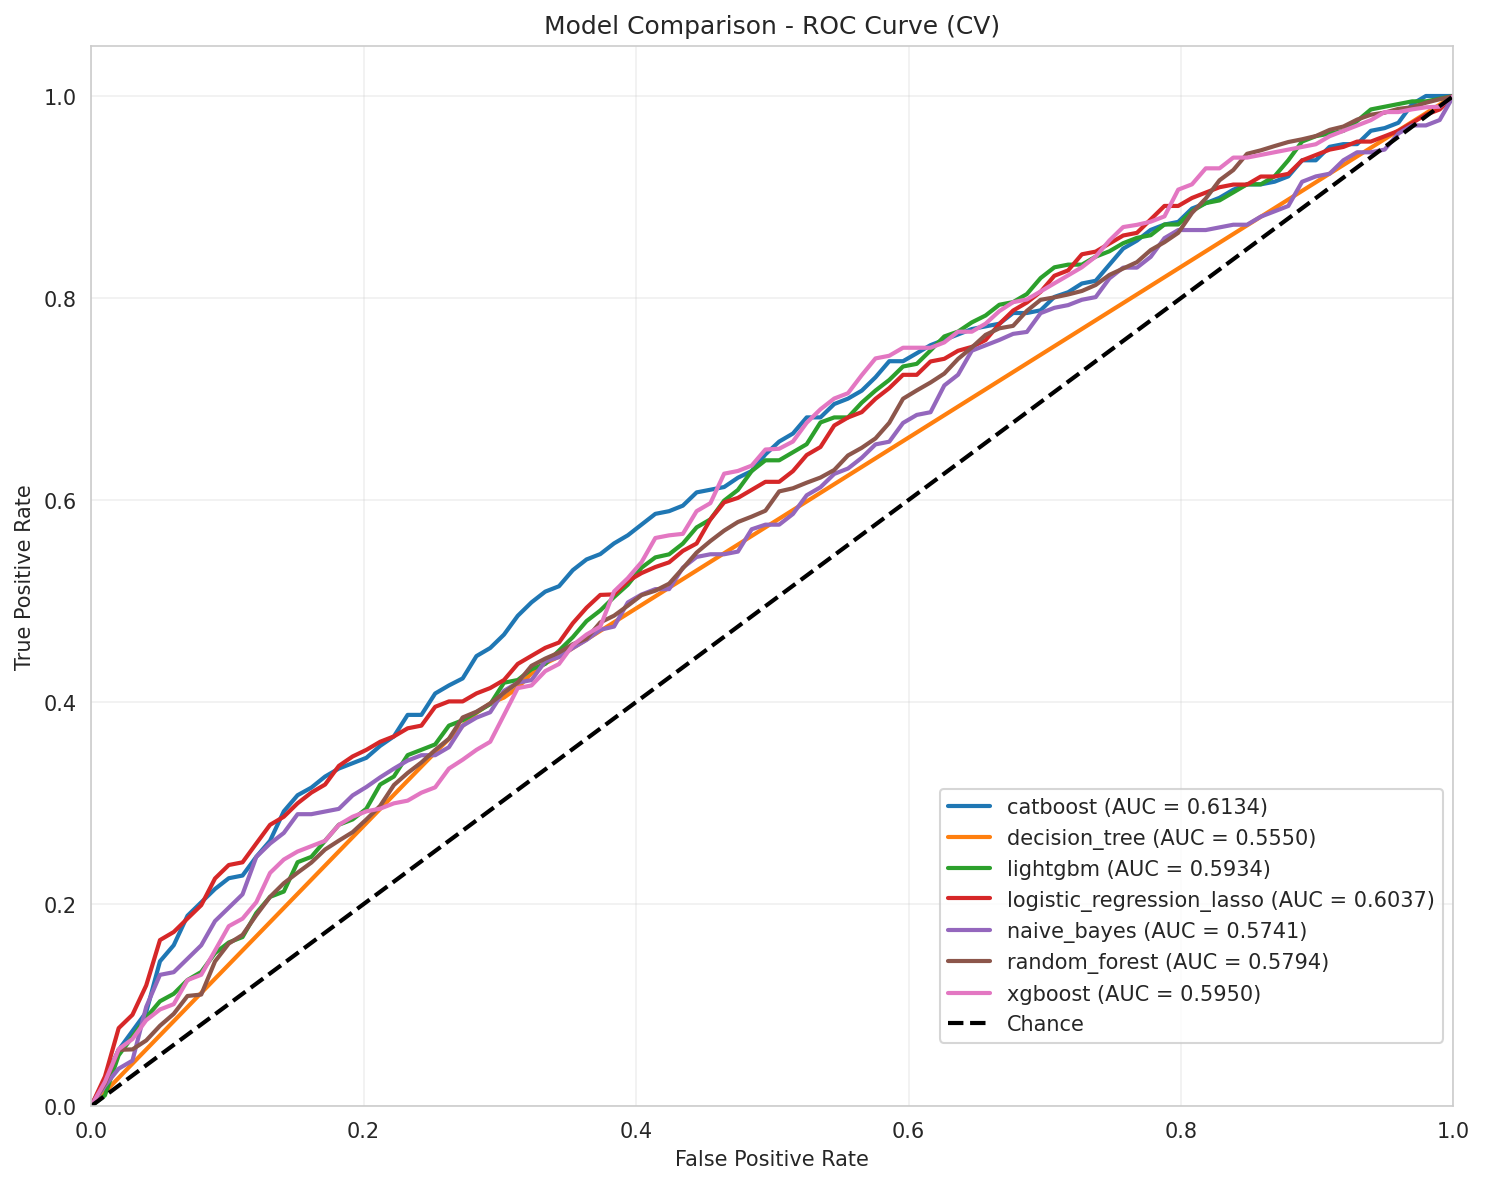
\includegraphics[width=0.85\textwidth]{../experiments/exp_03_categorical_features/comparison_plots/roc_comparison.png}
\caption{Comparacion ROC global del Experimento 3}
\label{fig:exp3-roc}
\end{figure}

\begin{figure}[H]
\centering
\includegraphics[width=0.78\textwidth]{../experiments/exp_03_categorical_features/models/catboost/plots/feature_importance.png}
\caption{Importancia de variables del modelo lider (catboost) en el Experimento 3}
\label{fig:exp3-fi-catboost}
\end{figure}

\subsection{Experimento 4: Pruning}

La tercera fase se enfoco en reducir ruido y mantener solo caracteristicas con mayor utilidad predictiva. En este escenario, catboost volvio a liderar con AUC-ROC de 0.6209.

\begin{table}[H]
\centering
\caption{Top 4 modelos por AUC-ROC en el Experimento 4}
\label{tab:exp4-top4}
\begin{tabular}{|l|c|}
\hline
\textbf{Modelo} & \textbf{AUC-ROC} \\ \hline
catboost & 0.6209 \\ \hline
logistic\_regression\_lasso & 0.6043 \\ \hline
xgboost & 0.6040 \\ \hline
random\_forest & 0.6032 \\ \hline
\end{tabular}
\end{table}

\begin{figure}[H]
\centering
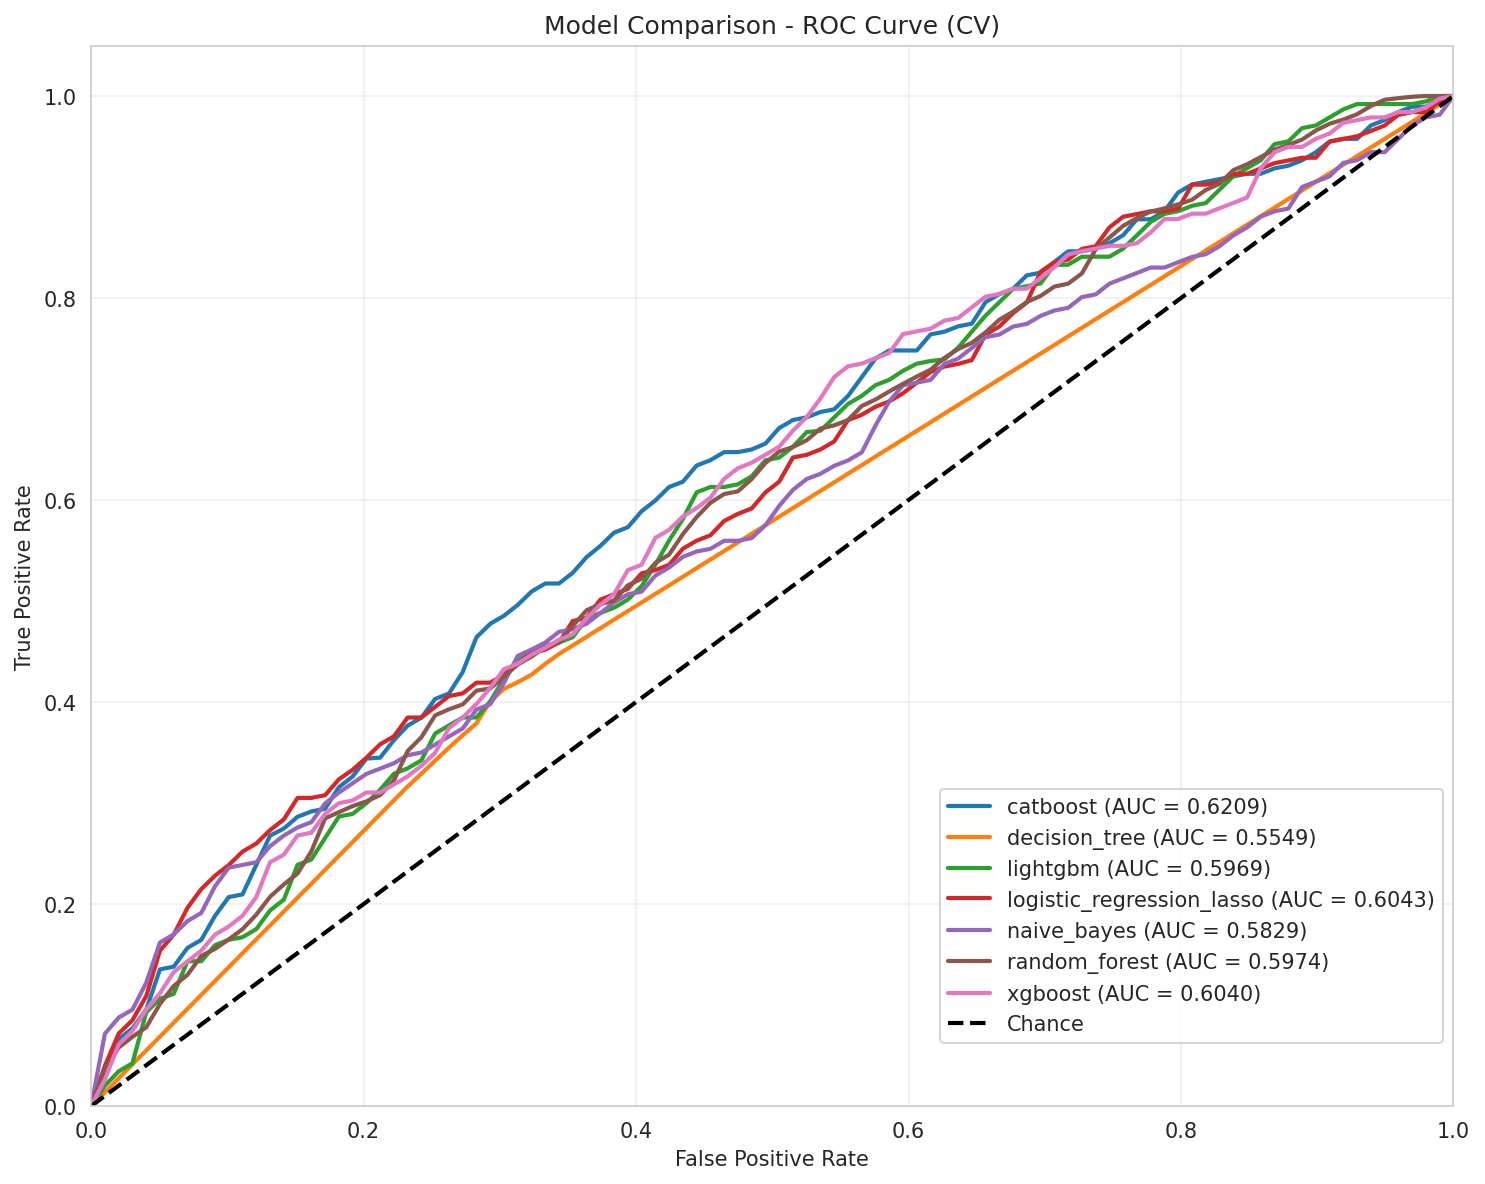
\includegraphics[width=0.85\textwidth]{../experiments/exp_04_feature_pruning/comparison_plots/roc_comparison.png}
\caption{Comparacion ROC global del Experimento 4}
\label{fig:exp4-roc}
\end{figure}

\begin{figure}[H]
\centering
\includegraphics[width=0.78\textwidth]{../experiments/exp_04_feature_pruning/models/catboost/plots/roc_curve_cv.png}
\caption{Curva ROC en CV del modelo lider (catboost) en el Experimento 4}
\label{fig:exp4-catboost-roc}
\end{figure}

\subsubsection{Comparativa complementaria en pruning}

Para reproducir el analisis de la presentacion, se incorpora la comparativa visual de curvas ROC en CV para los contendientes logistic\_regression\_lasso y xgboost bajo el mismo esquema de poda.

\begin{figure}[H]
\centering
\includegraphics[width=0.78\textwidth]{../experiments/exp_04_feature_pruning/models/logistic_regression_lasso/plots/roc_curve_cv.png}
\caption{Curva ROC en CV para logistic\_regression\_lasso en el Experimento 4}
\label{fig:exp4-lasso-roc}
\end{figure}

\begin{figure}[H]
\centering
\includegraphics[width=0.78\textwidth]{../experiments/exp_04_feature_pruning/models/xgboost/plots/roc_curve_cv.png}
\caption{Curva ROC en CV para xgboost en el Experimento 4}
\label{fig:exp4-xgb-roc}
\end{figure}

\subsection{Experimento 5: Hiperparametros}

La fase final realizo optimizacion de hiperparametros para todos los modelos y consolido la comparacion final de desempeno.

\begin{table}[H]
\centering
\caption{Ranking de modelos por AUC-ROC en el Experimento 5}
\label{tab:exp5-ranking}
\begin{tabular}{|c|l|c|}
\hline
\textbf{Ranking} & \textbf{Modelo} & \textbf{AUC-ROC} \\ \hline
1 & xgboost & 0.6391 \\ \hline
2 & random\_forest & 0.6356 \\ \hline
3 & lightgbm & 0.6338 \\ \hline
4 & decision\_tree & 0.6227 \\ \hline
5 & catboost & 0.6202 \\ \hline
6 & logistic\_regression\_lasso & 0.6133 \\ \hline
7 & naive\_bayes & 0.5840 \\ \hline
\end{tabular}
\end{table}

\begin{figure}[H]
\centering
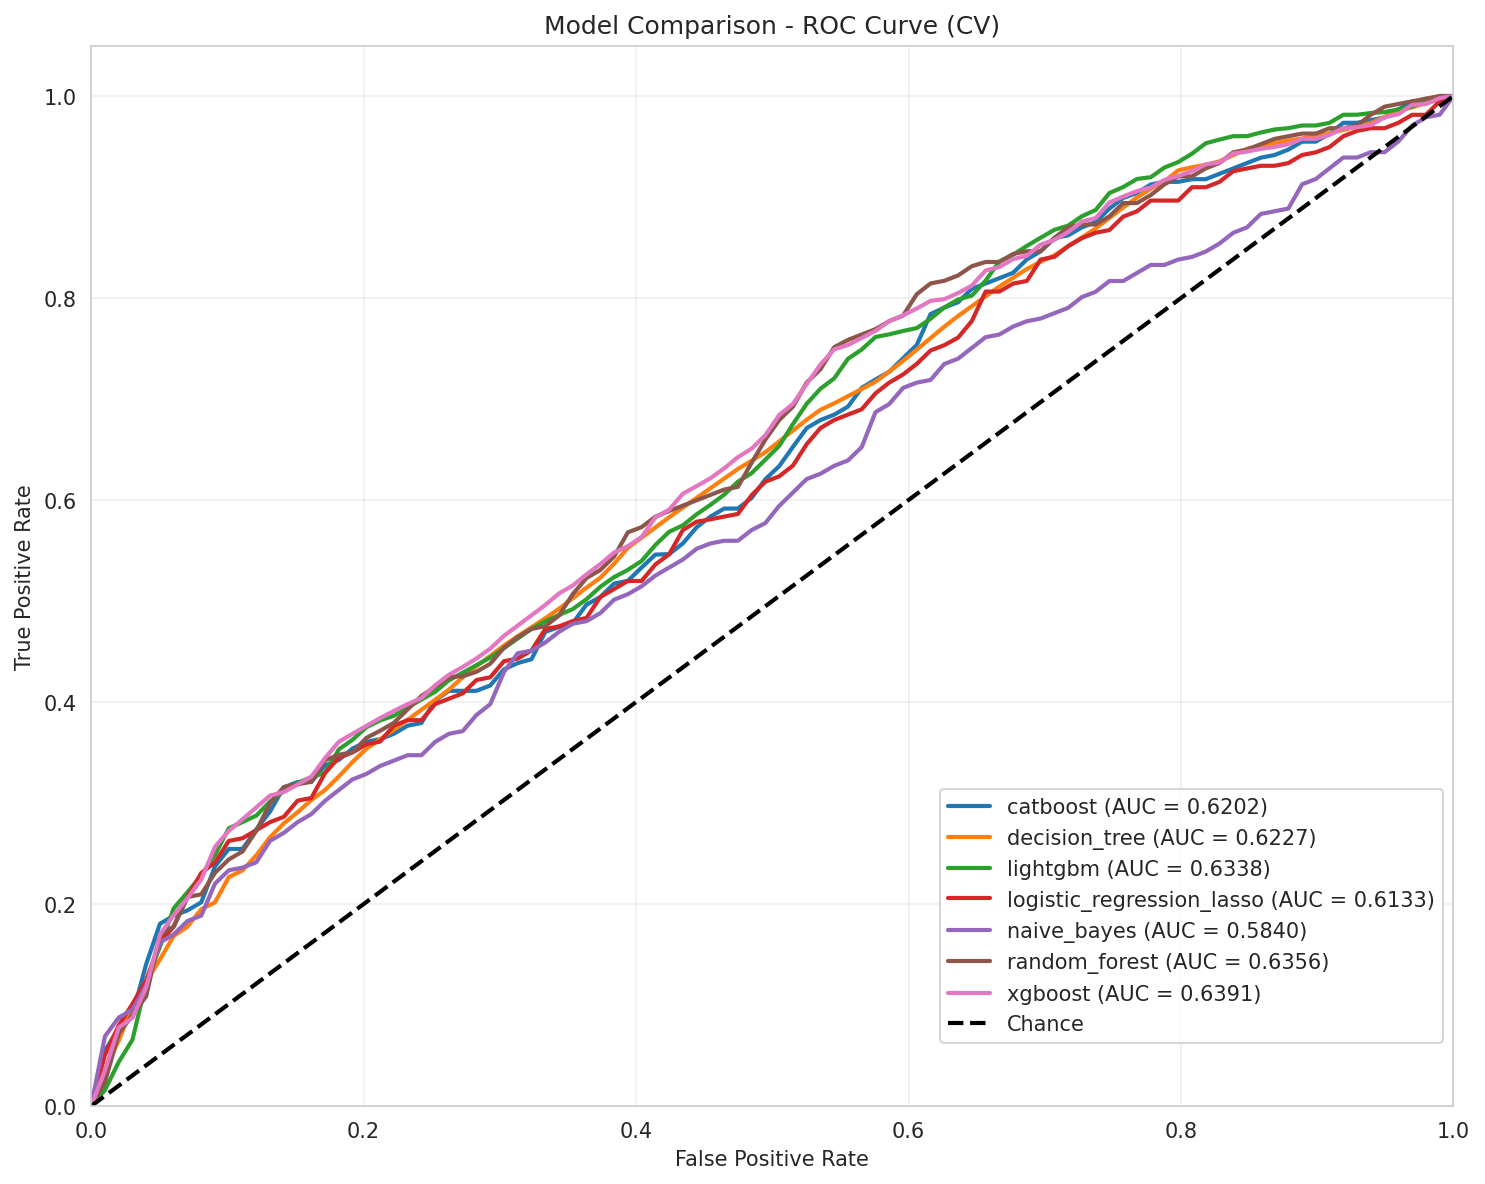
\includegraphics[width=0.85\textwidth]{../experiments/exp_05_hyperparameter_search/comparison_plots/roc_comparison.png}
\caption{Comparacion ROC global del Experimento 5}
\label{fig:exp5-roc}
\end{figure}

\begin{figure}[H]
\centering
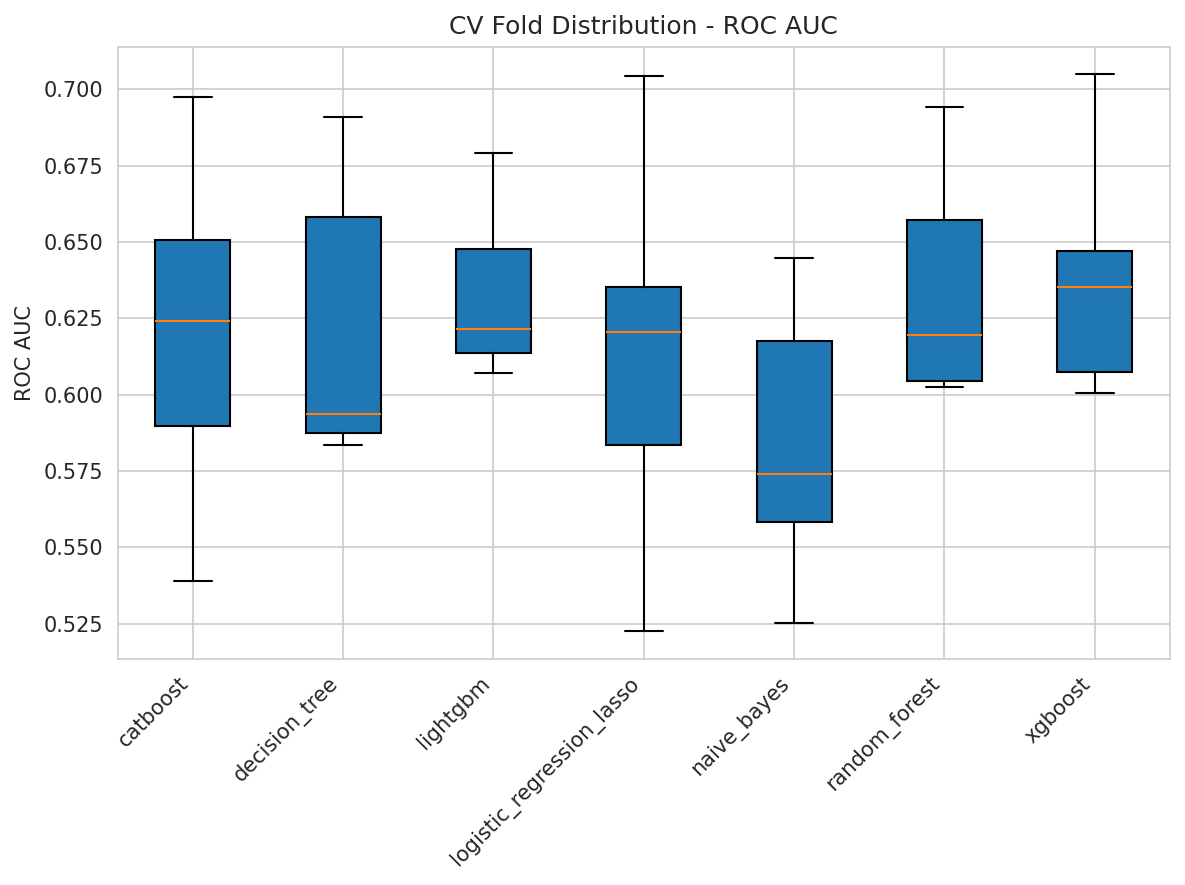
\includegraphics[width=0.85\textwidth]{../experiments/exp_05_hyperparameter_search/comparison_plots/roc_boxplot_comparison.png}
\caption{Distribucion de AUC-ROC por validacion cruzada para todos los modelos en el Experimento 5}
\label{fig:exp5-roc-boxplot}
\end{figure}

\begin{figure}[H]
\centering
\includegraphics[width=0.78\textwidth]{../experiments/exp_05_hyperparameter_search/models/xgboost/plots/feature_importance.png}
\caption{Importancia de variables del modelo lider (xgboost) en el Experimento 5}
\label{fig:exp5-xgb-fi}
\end{figure}

\subsubsection{Comparativa final: XGBoost vs Decision Tree}

Para la decision final se contrasto el mejor modelo discriminativo (xgboost) frente al mejor candidato interpretable (decision\_tree), usando las metricas de operacion reportadas en \texttt{plot\_metadata.json}.

\begin{table}[H]
\centering
\caption{Comparativa de metricas operativas en el Experimento 5}
\label{tab:exp5-duelo}
\begin{tabular}{|l|c|c|}
\hline
\textbf{Metrica} & \textbf{xgboost} & \textbf{decision\_tree} \\ \hline
AUC-ROC (CV) & 0.6391 & 0.6227 \\ \hline
Threshold optimo & 0.48 & 0.22 \\ \hline
Recall & 0.8647 & 0.8329 \\ \hline
Specificity & 0.2854 & 0.3304 \\ \hline
Precision & 0.3634 & 0.3698 \\ \hline
NPV & 0.8172 & 0.8073 \\ \hline
F1-score & 0.5118 & 0.5122 \\ \hline
F2-score & 0.6778 & 0.6661 \\ \hline
Accuracy & 0.4711 & 0.4915 \\ \hline
Kappa & 0.1100 & 0.1227 \\ \hline
\end{tabular}
\end{table}

Desde el criterio clinico de deteccion temprana, xgboost se prioriza por mayor recall y mayor AUC-ROC. En paralelo, decision\_tree conserva valor practico por su mejor especificidad y mayor interpretabilidad para discusion con equipo medico.

\begin{figure}[H]
\centering
\includegraphics[width=0.78\textwidth]{../experiments/exp_05_hyperparameter_search/models/xgboost/plots/roc_curve_cv.png}
\caption{Curva ROC en CV para xgboost (AUC=0.6391)}
\label{fig:exp5-xgb-roc}
\end{figure}

\begin{figure}[H]
\centering
\includegraphics[width=0.78\textwidth]{../experiments/exp_05_hyperparameter_search/models/decision_tree/plots/roc_curve_cv.png}
\caption{Curva ROC en CV para decision\_tree (AUC=0.6227)}
\label{fig:exp5-tree-roc}
\end{figure}

\subsubsection{Comparativas visuales del duelo final}

Adicionalmente se incluyen las mismas comparativas visuales presentadas en sustentacion para contrastar estabilidad y comportamiento operativo entre xgboost y decision\_tree.

\begin{figure}[H]
\centering
\includegraphics[width=0.78\textwidth]{../experiments/exp_05_hyperparameter_search/models/xgboost/plots/cv_fold_plots/cv_fold_roc_auc.png}
\caption{Boxplot de AUC-ROC por fold para xgboost en el Experimento 5}
\label{fig:exp5-xgb-cv-box}
\end{figure}

\begin{figure}[H]
\centering
\includegraphics[width=0.78\textwidth]{../experiments/exp_05_hyperparameter_search/models/decision_tree/plots/cv_fold_plots/cv_fold_roc_auc.png}
\caption{Boxplot de AUC-ROC por fold para decision\_tree en el Experimento 5}
\label{fig:exp5-tree-cv-box}
\end{figure}

\begin{figure}[H]
\centering
\includegraphics[width=0.78\textwidth]{../experiments/exp_05_hyperparameter_search/models/xgboost/plots/perf_precision_npv.png}
\caption{Comparativa precision-NPV para xgboost en el Experimento 5}
\label{fig:exp5-xgb-precision-npv}
\end{figure}

\begin{figure}[H]
\centering
\includegraphics[width=0.78\textwidth]{../experiments/exp_05_hyperparameter_search/models/decision_tree/plots/perf_precision_npv.png}
\caption{Comparativa precision-NPV para decision\_tree en el Experimento 5}
\label{fig:exp5-tree-precision-npv}
\end{figure}

\begin{figure}[H]
\centering
\includegraphics[width=0.78\textwidth]{../experiments/exp_05_hyperparameter_search/models/xgboost/plots/perf_f1_f2.png}
\caption{Comparativa F1-F2 para xgboost en el Experimento 5}
\label{fig:exp5-xgb-f1-f2}
\end{figure}

\begin{figure}[H]
\centering
\includegraphics[width=0.78\textwidth]{../experiments/exp_05_hyperparameter_search/models/decision_tree/plots/perf_f1_f2.png}
\caption{Comparativa F1-F2 para decision\_tree en el Experimento 5}
\label{fig:exp5-tree-f1-f2}
\end{figure}

\begin{figure}[H]
\centering
\includegraphics[width=0.78\textwidth]{../experiments/exp_05_hyperparameter_search/models/xgboost/plots/kappa.png}
\caption{Kappa para xgboost en el Experimento 5}
\label{fig:exp5-xgb-kappa}
\end{figure}

\begin{figure}[H]
\centering
\includegraphics[width=0.78\textwidth]{../experiments/exp_05_hyperparameter_search/models/decision_tree/plots/kappa.png}
\caption{Kappa para decision\_tree en el Experimento 5}
\label{fig:exp5-tree-kappa}
\end{figure}

\begin{figure}[H]
\centering
\includegraphics[width=0.78\textwidth]{../experiments/exp_05_hyperparameter_search/models/xgboost/plots/confusion_matrix_normalized.png}
\caption{Matriz de confusion normalizada para xgboost en el Experimento 5}
\label{fig:exp5-xgb-confusion}
\end{figure}

\begin{figure}[H]
\centering
\includegraphics[width=0.78\textwidth]{../experiments/exp_05_hyperparameter_search/models/decision_tree/plots/confusion_matrix_normalized.png}
\caption{Matriz de confusion normalizada para decision\_tree en el Experimento 5}
\label{fig:exp5-tree-confusion}
\end{figure}

\subsection{Evolucion global y cierre de fase experimental}

\begin{table}[H]
\centering
\caption{Evolucion del mejor AUC-ROC por experimento}
\label{tab:evolucion-auc}
\begin{tabular}{|l|c|c|}
\hline
\textbf{Experimento} & \textbf{Mejor modelo} & \textbf{AUC-ROC} \\ \hline
Exp 1 (Baseline) & catboost & 0.6153 \\ \hline
Exp 2 (Features agregadas) & catboost & 0.6235 \\ \hline
Exp 3 (Variables categoricas) & catboost & 0.6134 \\ \hline
Exp 4 (Feature pruning) & catboost & 0.6209 \\ \hline
Exp 5 (Hyperparameter search) & xgboost & 0.6391 \\ \hline
\end{tabular}
\end{table}

En terminos absolutos, la mejora del mejor modelo entre el inicio y el cierre experimental fue:

$$\Delta AUC = 0.6391 - 0.6153 = 0.0238$$

Adicionalmente, el modelo interpretable \texttt{decision\_tree} paso de AUC=0.5560 en Exp 1 a AUC=0.6227 en Exp 5, con una mejora absoluta de 0.0667.
